\subsection{\texorpdfstring{W+jets Background Estimation in $\tauTau$ Channel}{W+jets Background Estimation in tau-tau Channel}}
\subsubsection{Method Description}
As shown in table~\ref{tbl:cutflowtable}, the number of W+jets events surviving 
the selection cuts are found to be zero in search \binone and it may suffer from the low statistics of the W+jets sample. In addition, we need to verify if the W+jets events are simulated well and agree with data.
 The statistical uncertainty on the yields for W+jets events can be improved by extracting 
the $\mttwo$ cut efficiency in a sample with more statistics. To make this sample, some cuts with small correlation on the search variables are 
relaxed. Various samples with different relaxed cuts are examined to check the idea of small correlation 
between search variable and relaxed cuts. In the next section, the validation of this method will be discussed.\\
When the cut efficiency for the $\mttwo$ variable is found, then it is multiplied by the W+jets 
yields before cutting on this variable. This means, according to table~\ref{tbl:cutflowtable}, the cut efficiency for 
$\mttwo$ found in a relaxed sample should be multiplied by 31.93 to get an 
estimate for the W+jets events in search \binone.\\
The systematics that can be assigned to this method is the maximum
variation of the estimations among those relaxed samples.
\subsubsection{Method Validation}
The idea is to check the effect of three set of cuts independently, 
on the \mttwo cut efficiency in search \binone. 
Therefore, starting with a baseline selection cuts, defined as two 
medium-isolated opposite sign \Tau's, the $\mttwo$ cut 
efficiency is calculated, for those events passing and failing the following list of cuts (one-by-one)
\begin{itemize}
\item lepton veto
\item $\mindphifour>$ 1
\item Z veto 
\end{itemize}

 The cut efficiencies and final estimated values for 
search \binone can be found in figure~\ref{fig:wjets_1}. These plots can be used to verify the method. 
\begin{figure}[iHhtb]
\centering
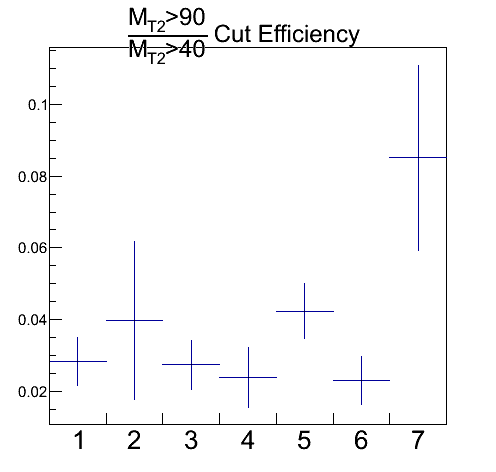
\includegraphics[angle=0,scale=0.35]{TauTauFigs/eff_bin1.png}
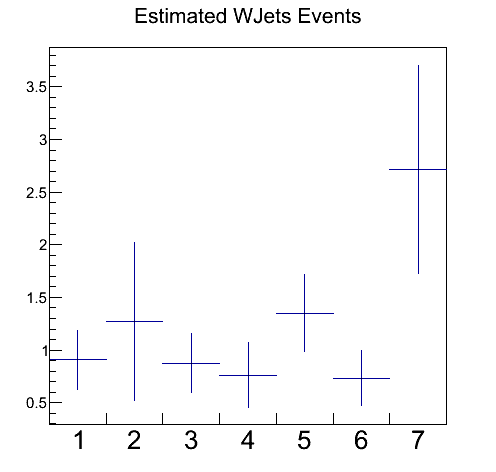
\includegraphics[angle=0,scale=0.35]{TauTauFigs/est_bin1.png} \\
\caption{The distribution of $\frac{\mttwo>90}{\mttwo>40}$ cut 
efficiency (left) and final estimated W+jets events (right) in search \binone.
 The first bin corresponds to the sample of events passing the baseline selection cuts. 
The next six bins correspond to the samples where passing and failing the 
list of cuts mentioned in the text, respectively.}
\label{fig:wjets_1}
\end{figure}

[{\bf FIXME} update the extracted values from the plots, according to the discussion in the SUSY meeting] A summary of the estimated W+jets events can be found in table~\ref{tbl:wjetsEstimation}. 

\begin{table}
\begin{center}
\begin{tabular}{lc}
\hline\hline
& W+jets Estimated Results\\
\hline
\binone & 0.66 $\pm$ 0.15 (stat.) $\pm$ 0.20 (sys.)\\
\hline\hline 
\end{tabular}
\caption{The W+jets estimation results. The systematics comes from the maximum variation of the estimations (neglecting the 7th bin) [{\bf FIXME} justify this with a plot: comment from SUSY meeting].}
\label{tbl:wjetsEstimation}
\end{center}
\end{table}

\subsubsection{MC Validation for W+jets}
To verify that the MC has a good description of the W+jets events and it can be trusted for both shape and normalization, a data/MC comparison 
is done in a W+jets enriched sample. To enrich the sample, \muTau selection is done with the following modifications:
\begin{itemize}
\item $\mu$ and \Tau are same sign.
\item B-tagged jets with CSVL are vetoed.
\item \Tau isolation changed from Tight to Loose.
\end{itemize}
Figure \ref{fig:mt2_WValidation} 
\begin{figure}[htbp]
\centering
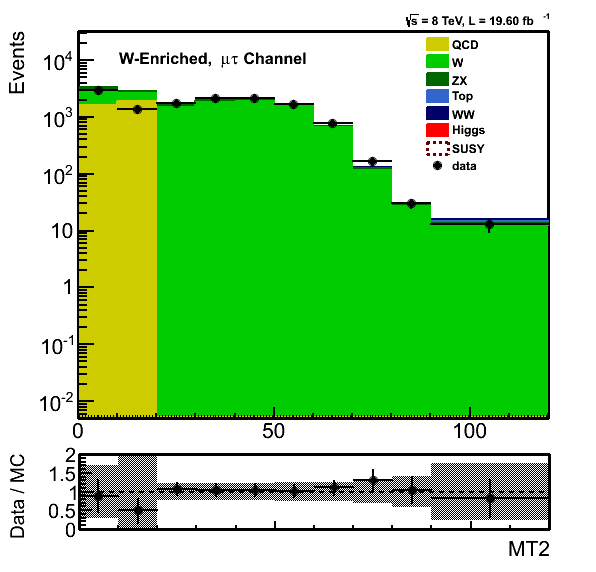
\includegraphics[angle=0,scale=0.35]{TauTauFigs/MT2_WValidation.png}
\caption{The \mttwo distribution in the W-Enriched region. Data and MC agree in both shape and normalization within the uncertainties.}
\label{fig:mt2_WValidation}
\end{figure}
shows the \mttwo distribution for the selected events. We use the range 40 $<\mttwo<$ 60 \GeV to find the normalization factor of the 
W+jets sample. In this range more than 90\% of the MC events are from the W+jets sample. 
All of the non-W MC events in this range are subtracted from 
the data in the same range. The result is compared with the MC prediction for the W+jets in this range. The k-factor for the W+jets sample is 
found to be 1.05 $\pm$ 0.13 which is compatibe with 1 within the errors. To evaluate the uncertainty, all of the statistical uncertaities on data 
and MC are considered plus 25\% systematic uncertainty on the MC samples.

To validate the shape of the W+jets sample, we compare the ratio of events with \mttwo $>$ 90 \GeV and  \mttwo $>$ 40 \GeV in data and MC.
The procedures to find the W+jets in data and consider the uncertainties are exactly same as the procdures for exctracting the normalization  
factor. This ratio is found to be 0.00213 $\pm$ 0.00086 in data and  0.0029 $\pm$ 0.0019 in MC. The values are consistent with each other within 
the considered uncertainties.

As the simulation of W+jets events agrees well with data, for the search \bintwo, the expected number of W+jets from MC which is $0.43\pm0.4$ is trusted and is used.

